\documentclass{standalone}
\usepackage{tikz}
\usepackage{ctex,siunitx}
\usepackage{tkz-euclide}
\usepackage{amsmath}
\usetikzlibrary{patterns, calc}
\usetikzlibrary {decorations.pathmorphing, decorations.pathreplacing, decorations.shapes,}
\begin{document}
\small
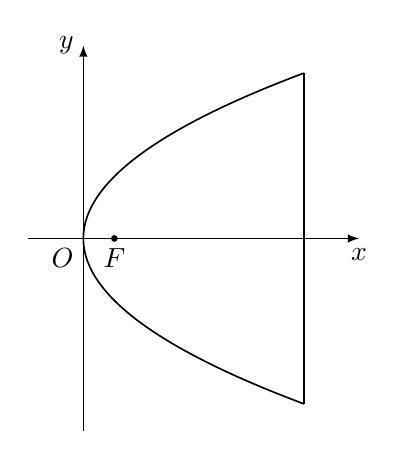
\begin{tikzpicture}[>=latex,scale=0.07]
  \draw[thin,->](-10,0)--(50,0)node[below]{$x$};
  \draw[thin,->](0,-35)--(0,35)node[left]{$y$};
  \tkzDefPoints{0/0/O,5.625/0/F}
  \draw[semithick,samples=200,domain=-30:30] plot ({2*\x*\x/45},{\x});
  \draw[semithick](40,30)--(40,-30);
  \tkzDrawPoints[fill=black](F)
  \tkzLabelPoints[below left](O)
  \tkzLabelPoints[below](F)
\end{tikzpicture}
\end{document}